\section{Asynchronous Reinforcement Learning with Single Rollout}
% In this section, We propose a Single-Rollout Asynchronous RL framework designed to maximize training throughput by removing the computational overhead of group-wise sampling. While efficient, single-rollout training introduces high gradient variance and policy lag. To resolve this, we present three technical contributions. First, we formulate a simplified importance sampling objective that directly utilizes rollout logs, avoiding the cost of synchronized reference models. Second, we stabilize value model training through a faster-critic-update technique and an attention-freezing strategy. Third, we derive a Skip-Observation GAE formulation to correct advantage estimation in multi-turn agentic trajectories.

\begin{figure}
    \centering
    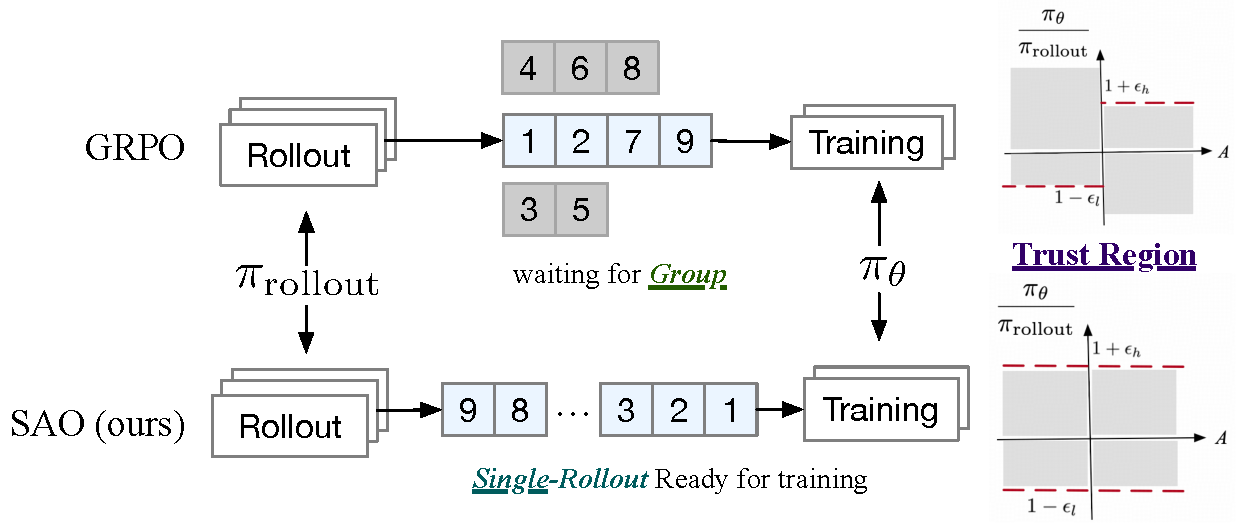
\includegraphics[width=0.7\linewidth]{figures/overview.pdf}
    \caption{Overview of \model with single rollout design. The numbers denote the generation order of trajectories. For \model, each trajectory becomes available for training immediately upon completion. In contrast, GRPO must wait until all trajectories in a group are generated before training can begin.}
    \label{fig:overview}
\end{figure}

In this section, we introduce \model to tackle training instability and off-policy drift in asynchronous RL training. With a simple token-level clipping strategy and single rollout as an alternative to group-wise sampling, we show that asynchronous RL can be stably scaled to thousands of training steps and achieve significant performance improvements. Figure~\ref{fig:overview} shows the overall design of \model.

\subsection{Stabilizing Asynchronous RL via Direct Double-Sided Importance Sampling (DIS) }

A primary challenge in asynchronous RL is the ``policy lag'' that emerges between rollout models and the training models. In decoupled PPO for LLM, importance sampling is employed to relieve off-policy bias by keeping three distinct models: the current policy $\pi_{\theta}$, the old policy $\pi_{\theta_{\text{old}}}$, and the rollout policy $\pi_{\text{rollout}}$, where $\frac{\pi_{\theta}}{\pi_{\theta_{\text{old}}}}$ is used for staled off-policy correction and $\frac{\pi_{\theta_{\text{old}}}}{\pi_{\text{rollout}}}$ for training-rollout mismatch.
However, as rollout engines may undergo multiple updates during a single trajectory generation in asynchronous RL,
this renders the tracking of exact behavior probabilities $\pi_{\theta_{\text{old}}}$ computationally prohibitive. Otherwise, we have to maintain an extensive history of model checkpoints $\{\pi_{\theta_{\text{old}}^{(1)}}, \dots, \pi_{\theta_{\text{old}}^{(N)}}\}$, which is infeasible in practical implementation.

To resolve this, we propose a simplified yet aggressive token-level importance sampling to clip off-policy tokens.
First, we directly use $\pi_{\text{rollout}}$ as the behavior proxy and $\pi_{\theta}$ for importance sampling, i.e., $r_t(\theta)=\frac{\pi_{\theta}}{\pi_{\text{rollout}}}$, while dropping the inaccurate $\pi_{\theta_{\text{old}}}$. This eliminates the computational overhead of separate old-policy inference by utilizing the log-probabilities generated during the rollout phase.

Second, we employ a double-sided calibration token-level masking strategy. Unlike standard PPO clipping, which clips only selected off-policy tokens with $(A>0, r_t(\theta) > 1+\epsilon_h)$ or $(A<0, r_t(\theta)<1-\epsilon_l)$, we restrict the trust region to the interval $[1-\epsilon_\ell, 1+\epsilon_h]$, while tokens falling outside this range are masked from gradient computation entirely to prevent instabilities arising from extreme policy divergence. This shares similarities with the IcePop mechanism \cite{team2025every}, yet our strategy is simpler by further removing $\pi_{\theta_{\text{old}}}$ while still achieving stable training.

Formally, the optimization objective with token-level clipping can be written as:
\begin{equation}
    L(\theta) = \hat{\mathbb{E}}_t \left[ f(r_t(\theta), \epsilon_l, \epsilon_h) \hat{A}_t \log \pi_{\theta}(a_t|s_t) \right]
\end{equation}
In this formulation, the probability ratio $r_t(\theta)$ is computed directly from the rollout logs to circumvent the need for historical policy tracking:
\begin{equation}
    r_t(\theta) = \exp\left( \log \pi_\theta(a_t|s_t) - \log \pi_{\text{rollout}}(a_t|s_t) \right)
\end{equation}
Stability is further enforced via the calibration function $f(x; \epsilon_\ell, \epsilon_h)$:
\begin{equation}
    f(x; \epsilon_\ell, \epsilon_h) = 
    \begin{cases} 
    x, & \text{if } 1-\epsilon_\ell < x < 1+\epsilon_h \\
    0, & \text{otherwise}
    \end{cases}
\end{equation}


This design circumvents the intensive need to track the historical model ensemble. By utilizing the rollout log-probabilities directly, we accept a controlled degree of off-policy bias in exchange for a substantial reduction in computational complexity and the elimination of errors associated with using a single, potentially stale, ``latest'' old policy model. Empirical results demonstrate that this simplified mechanism enables more aggressive clipping, which effectively regularizes the update steps and yields superior training stability in asynchronous settings.




\subsection{Reducing Off-Policy with Single Rollout}
In asynchronous RL, an inevitable problem is off-policy. Yet current popular group-wise sampling RL algorithms, e.g., GRPO, could introduce more severe off-policy.
Group-wise sampling introduces an ``imbalanced generation'' bias, and the group data has to wait for the ``slowest'' sample to finish before being fed into training.
One promising solution is to replace group-wise sampling with single-rollout, where a sample is immediately fed into training upon generation.

However, single-rollout optimization inherently suffers from high variance in gradient estimation, similar to REINFORCE~\cite{zhang2021sample}. To reduce variance requires a sufficiently good value model. In this part, we focus on simple strategies to optimize value modeling to ultimately boost the policy's performance.  

\vpara{Faster Value Update than Policy.}
We identify that the primary source of instability in single-rollout RL is the interdependence between the policy and the value function. If the value model $V_\phi$ is inaccurate, the advantage estimates $\hat{A}_t$ become noisy, leading to destructive policy updates.
To mitigate this, we implement a Faster Value Update adapted for LLMs. We decouple the optimization frequencies of the policy and the value model. Specifically, for every single gradient update applied to the policy $\pi_{\theta}$, we enforce $K$ updates to the value network $V_{\phi}$ (where $K > 1$).
% \hide{
% \begin{align*}
%     \phi_{t+1} &\leftarrow \text{Optimizer}_V(\phi_t, \nabla L_V, K \text{ steps}) \\
%     \theta_{t+1} &\leftarrow \text{Optimizer}_\pi(\theta_t, \nabla L_\pi, 1 \text{ step})
% \end{align*}
% }
In our experiments, we set $K=2$. This strategy facilitates the faster adaptation of value estimates to the current policy before they are utilized for advantage computation, thereby reducing the variance.

\vpara{Stabilizing Value Model Training via Parameter Freezing.}
In our pilot experiments, we find the instability of value model training, where the gradient norms of the value model are significantly larger than the corresponding policy model. Further decomposition shows that this instability originates primarily from the Full Attention layers, whereas the Mixture-of-Experts (MoE) layers remain relatively stable.
Based on this observation, we employ a ``Frozen-Attention'' training strategy for the value model. During the RL training, we freeze the parameters of the attention modules in $V_\phi$ and optimize the MoE projections.
We hypothesize that the pre-trained attention weights already possess sufficient semantic capability to attend to relevant tokens. By restricting optimization to the MoE layers, we effectively regularize the value model.
% preventing overfitting to transient high-variance reward signals while retaining the capacity to map semantic states to scalar values.

\vpara{Skip-Observation Token-level GAE for Agentic Tasks.}
Agentic tasks present a unique challenge for token-level value estimation due to their trajectory structure: $T = [a_0, o_0, a_1, o_1, \dots]$, where $a_i$ represents model actions and $o_i$ represents environment feedback. Standard Generalized Advantage Estimation (GAE) attempts to calculate the value difference between adjacent tokens. However, the transition from the end of an action $a_{i, \text{end}}$ to the start of an observation $o_{i, \text{start}}$ is discontinuous from the model's perspective, as the model does not generate $o_i$.
Calculating advantage across this boundary introduces noise, as the value model $V(o_{i, \text{start}})$ attempts to predict the value of an external environment state.

To resolve this, we derive a ``Skip-Observation'' GAE. We explicitly modify the Bellman target to bypass environment feedback tokens, linking the value of the current action directly to the value of the subsequent action.
Formally, let $a_{i, N}$ be the last token of action $i$, and $a_{i+1, 0}$ be the first token of the next action. We define the advantage as:

\begin{equation}
    \hat{A}(a_{i, N}) = \delta + \gamma \lambda \hat{A}(a_{i+1, 0})
\end{equation}

where the temporal difference residual $\delta$ is calculated bridging the observation gap:

\begin{equation}
    \delta = r_t + \gamma V(a_{i+1, 0}) - V(a_{i, N})
\end{equation}

This formulation constrains the advantage estimation to rely purely on the model outputs, filtering out the stochasticity of environment feedback. In contrast, some works may consider using a step-level value function and GAE as an alternative to the token-level value; however, we found that a step-level value could lead to suboptimal performance, which will be shown in the experimental part.
We also conduct other advantage designs for agentic traces, and the results can be found in the Appendix. 

\vpara{Scaling Value Pretraining.}
Finally, to support these mechanisms, we find it essential to scale the data used for value model pretraining. Our experiments demonstrate that the ``cold start'' problem in value estimation is a major bottleneck. By significantly increasing the scale of the value pretraining corpus, we provide a robust initialization point that promotes the effectiveness of our single-rollout and TTUR mechanisms from the early stages of training.


